\section{Auswertung}
\label{sec:Auswertung}


\subsection{Ausgangssignal ohne Rauschen}
\label{sec:oR}
Die Graphen wurden sowohl mit Matplotlib \cite{matplotlib} als auch mit NumPy \cite{numpy} erstellt.
Der Oszillator-Ausgang liefert eine konstante Spannung von $\SI{11,5}{\volt}$.
Am Referenz-Ausgang lässt sich die Spannung regeln.

\begin{figure}
\centering
\begin{minipage}{0.48\textwidth}
\centering
\center{$\Delta\phi=\SI{0}{\degree}$}
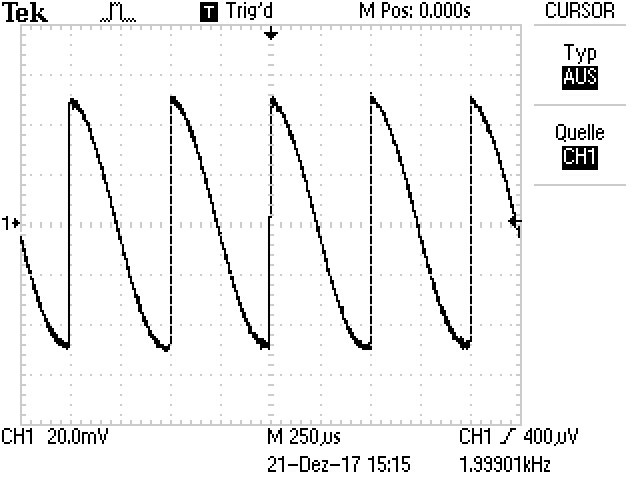
\includegraphics[scale=.75]{content/images/00.jpg}
\end{minipage}
\begin{minipage}{0.48\textwidth}
\centering
\center{$\Delta\phi=\SI{45}{\degree}$}
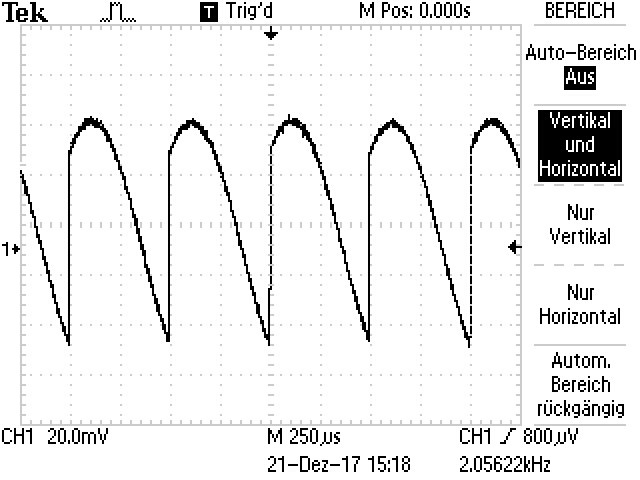
\includegraphics[scale=.75]{content/images/45.jpg}
\end{minipage}

\vspace{2em}
\begin{minipage}{0.48\textwidth}
\centering
\center{$\Delta\phi=\SI{90}{\degree}$}
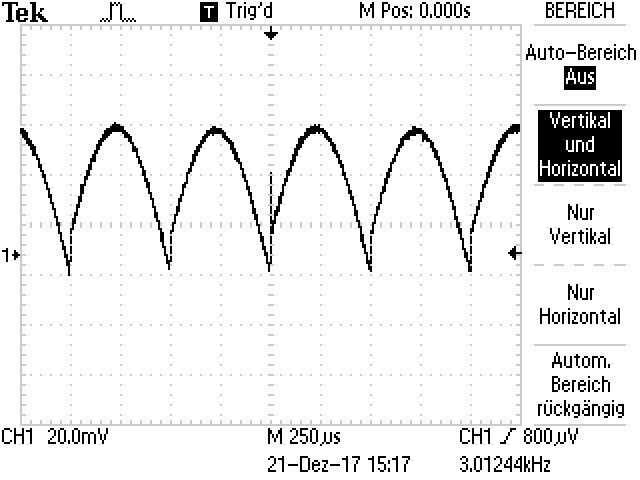
\includegraphics[scale=.75]{content/images/90.jpg}
\end{minipage}
\begin{minipage}{0.48\textwidth}
\centering
\center{$\Delta\phi=\SI{180}{\degree}$}
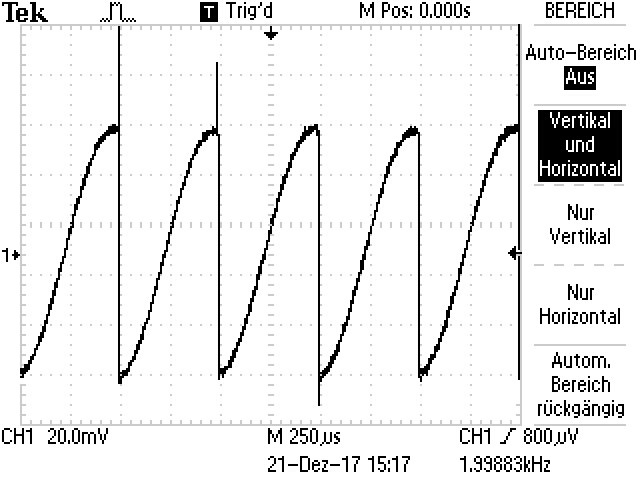
\includegraphics[scale=.75]{content/images/180.jpg}
\end{minipage}

\vspace{2em}
\begin{minipage}{.48\textwidth}
\centering
\center{$\Delta\phi=\SI{270}{\degree}$}
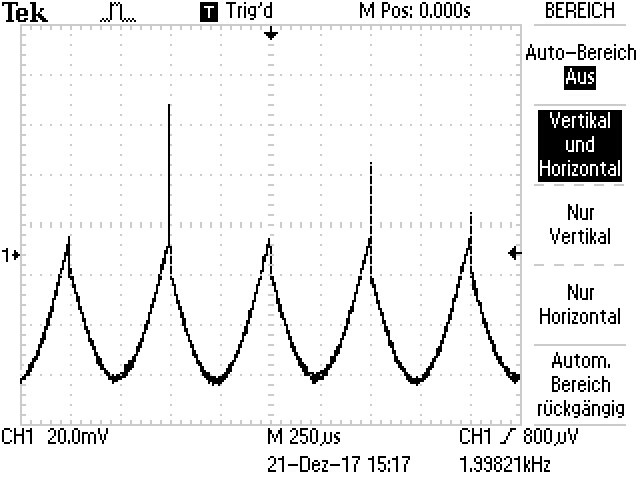
\includegraphics[scale=.75]{content/images/270.jpg}
\end{minipage}
\caption{Spannungsverläufe bei Phase $\Delta\phi$ ohne Tiefpassfilter und ohne Rauschen.}
\label{fig:U}
\end{figure}

\noindent Die Signal-Spannung $U_.{Sig}$ am Referenz-Ausgang wurde auf $\SI{10e-3}{\volt}$ bei $\SI{1000}{\hertz}$  und der Gain des Vorverstärkers auf 2 eingestellt. Als Referenzspannung $U_.{ref}$ wird die oben genannte Spannung des Oszillator-Ausgangs verwendet. Dessen Frequenz ist gleich der des Referenz-Ausgangs. In Abbildung \ref{fig:U} sind die Spannungsverläufe für verschiedene Phasenverschiebungen $\Delta\phi$ abgebildet.

\begin{table}
	\centering
	\caption{Messwerte der Ausgangsspannung $U_.{out}$ nach dem Tiefpassfilter ohne Rauschen.}
	\sisetup{table-format=1.2}
	\begin{tabular}{S[table-format=3.0] S[table-format=2.2]}
		\toprule
		{$\phi/\si{\degree}$}&{$U_.{out}/\si{\volt}$} \\
		\midrule
		45 & 2,52 \\
		90 & 4,08 \\
		105 & 4,16 \\
		135 & 3,32 \\
		150 & 2,16 \\
		180 & 0,44 \\
		225 & -2,68 \\
		270 & -4,08 \\
		315 & -3,24 \\
		360 & -0,45 \\
		\bottomrule
	\end{tabular}
	\label{tab:tab1}
\end{table}

\noindent Mit den Messwerten mit eingeschaltetem Tiefpassfilter aus Tabelle \ref{tab:tab1} wird die Regression
\begin{equation}
U_.{out}(\phi) = U_.{max}\cdot cos(f\cdot\phi+\phi_.0)\label{eq:Reg}
\end{equation}
durchgeführt:
\begin{align*}
U_.{max} &= \SI{4,13(5)}{\volt}, \\
f 		 &= (17,5\pm0,1)\cdot 10^{-3}, \\
\phi_.0  &= 1,47 \pm0,03 \text{.}\\
\end{align*}
Mit Gleichung \eqref{eq:} ergibt sich für die Theoriekurve:
\begin{align*}
U_.{max,theo} &= \SI{12,7e-3}{\volt}, \\
f_.{theo}	  &= \frac{\pi}{180} = 17,5 \cdot 10^{-3}, \\
\phi_.{0,theo}&= 0, \\
\end{align*}
wobei $f$ der Umrechnungsfaktor von Grad zu Bogenmaß ist.
Damit ergibt sich eine Abweichung von den experimentellen zu den theoretischen Werten von:
\begin{align*}
\Delta U_.{max} &= 32327\% ,\\
\Delta f		&= 0,00\% \text{.}\\
\end{align*}
Die Graphen dazu sind in Abbildung \ref{fig:U2} zu sehen.

\begin{figure}
\centering
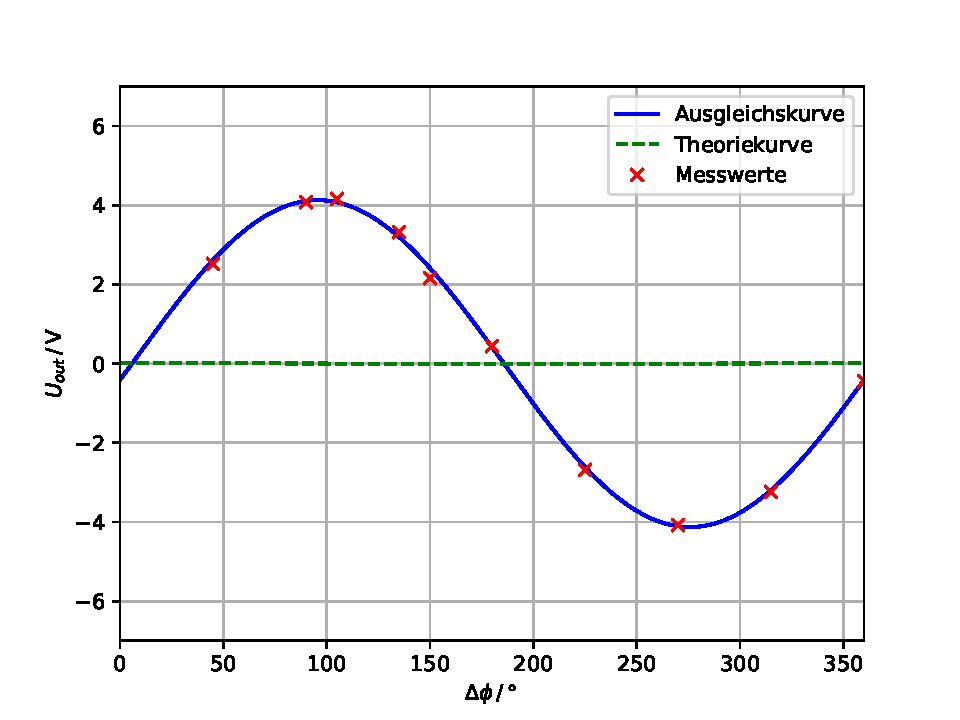
\includegraphics[width=\linewidth-75pt,height=\textheight-75pt,keepaspectratio]{content/images/plot.pdf}
\caption{Graphen der Messwerte mit Tiefpassfilter und ohne Rauschen.}
\label{fig:U2}
\end{figure}


\subsection{Ausgangssignal mit Rauschen}
\label{sec:mR}
Der Rauschgenerator ist auf $10^{-3}$ gestellt. Die Spannungsverläufe für verschiedene Phasendifferenzen sind in Abbildung \ref{fig:U3} dargestellt.

\begin{figure}
\centering
\begin{minipage}{0.48\textwidth}
\centering
\center{$\Delta\phi=\SI{0}{\degree}$}
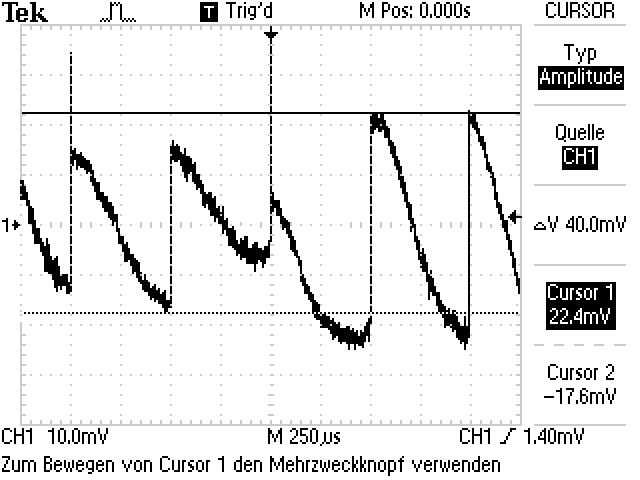
\includegraphics[scale=0.75]{content/images/noise0.jpg}
\end{minipage}
\begin{minipage}{0.48\textwidth}
\centering
\center{$\Delta\phi=\SI{45}{\degree}$}
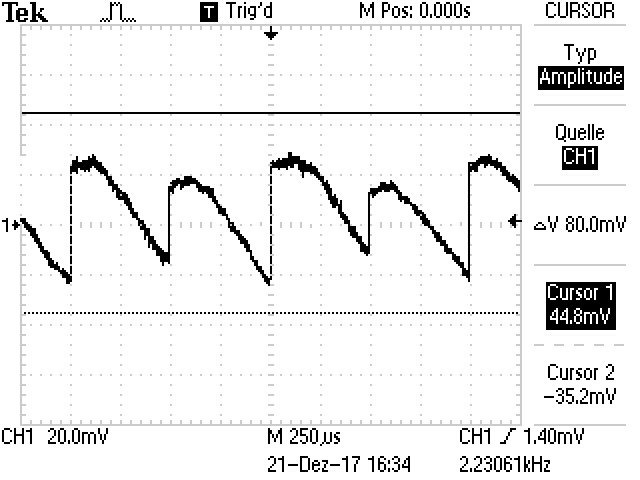
\includegraphics[scale=0.75]{content/images/noise45.jpg}
\end{minipage}

\vspace{2em}
\begin{minipage}{0.48\textwidth}
\centering
\center{$\Delta\phi=\SI{90}{\degree}$}
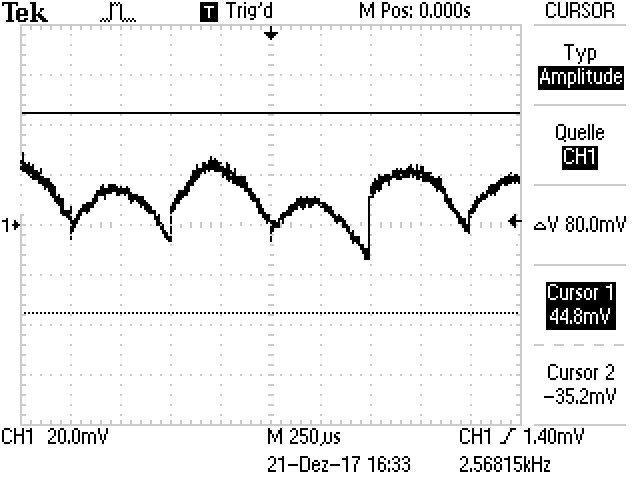
\includegraphics[scale=0.75]{content/images/noise90.jpg}
\end{minipage}
\begin{minipage}{0.48\textwidth}
\centering
\center{$\Delta\phi=\SI{180}{\degree}$}
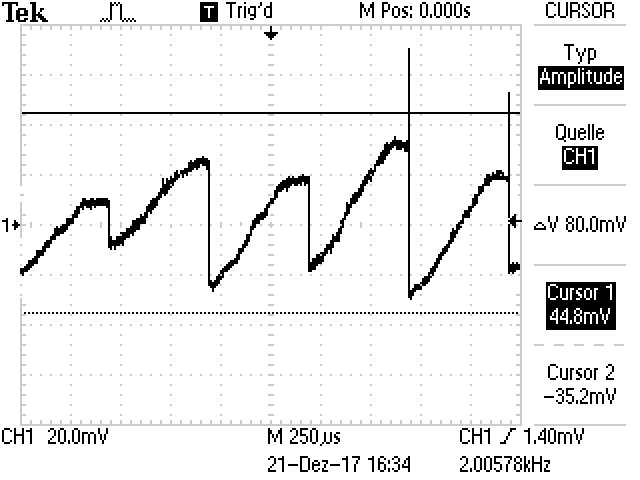
\includegraphics[scale=0.75]{content/images/noise180.jpg}
\end{minipage}

\vspace{2em}
\begin{minipage}{0.48\textwidth}
\centering
\center{$\Delta\phi=\SI{270}{\degree}$}
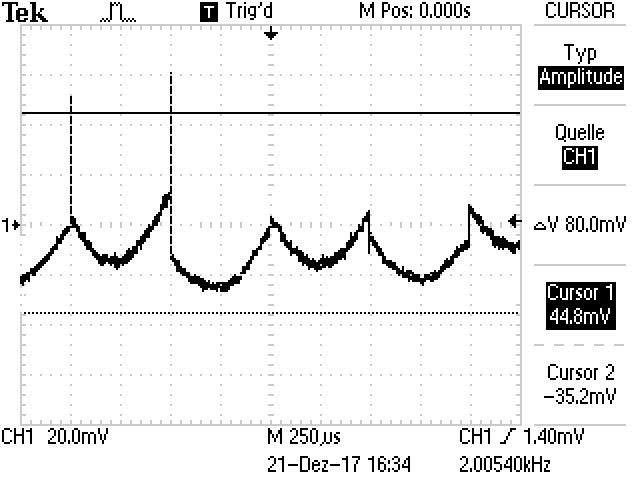
\includegraphics[scale=0.75]{content/images/noise270.jpg}
\end{minipage}
\caption{Spannungsverläufe bei Phase $\Delta\phi$ ohne Tiefpassfilter mit Rauschen.}
\label{fig:U3}
\end{figure}

\begin{table}
	\centering
	\caption{Messwerte der Ausgangsspannung $U_.{out}$ nach dem Tiefpassfilter mit Rauschen.}
	\sisetup{table-format=1.2}
	\begin{tabular}{S[table-format=3.0] S[table-format=3.1]}
		\toprule
		{$\phi/\si[per-mode=reciprocal]{\degree}$}&{$U_.{out}/10^{-3}\si[per-mode=reciprocal]{\volt}$} \\
		\midrule
		45 & 34,4 \\
		90 & 59,2 \\
		105 & 60,8 \\
		135 & 52,8 \\
		150 & 34,4 \\
		180 & 13,0 \\
		225 & -32,8 \\
		270 & -56,0 \\
		315 & -48,0 \\
		360 & -11,4 \\
		\bottomrule
	\end{tabular}
	\label{tab:tab2}
\end{table}

\noindent Die Messwerte nach Zuschalten des Tiefpassfilters und Erhöhung des Vorverstärker-Gains auf 10 sind in Tabelle \ref{tab:tab2} zu sehen. Damit wird wird die lineare Regression nach Gleichung \eqref{eq:Reg} durchgeführt.
Es ergeben sich:
\begin{align*}
U_.{max} &= \SI{5,9(1)e-2}{\volt} ,\\
f 		 &= (17,4\pm0,1)\cdot 10^{-3} ,\\
\phi_.0  &= 1,40\pm0,05 \text{.}\\
\end{align*}
Mit Gleichung \eqref{eq:} ergibt sich für die Theoriekurve:
\begin{align*}
U_.{max,theo} &= \SI{6,3e-2}{\volt} ,\\
f_.{theo}	  &= 17,5\cdot 10^{-3} ,\\
\phi_.{0,theo}&= 0 \text{.}\\
\end{align*}
Damit ergeben sich die Abweichungen:
\begin{align*}
\Delta U_.{max} &= 6,79\% ,\\
\Delta f		&= 0,29\% \text{.}\\
\end{align*}
Die Graphen dazu sind in Abbildung \ref{fig:U4} zu sehen.

\begin{figure}
\centering
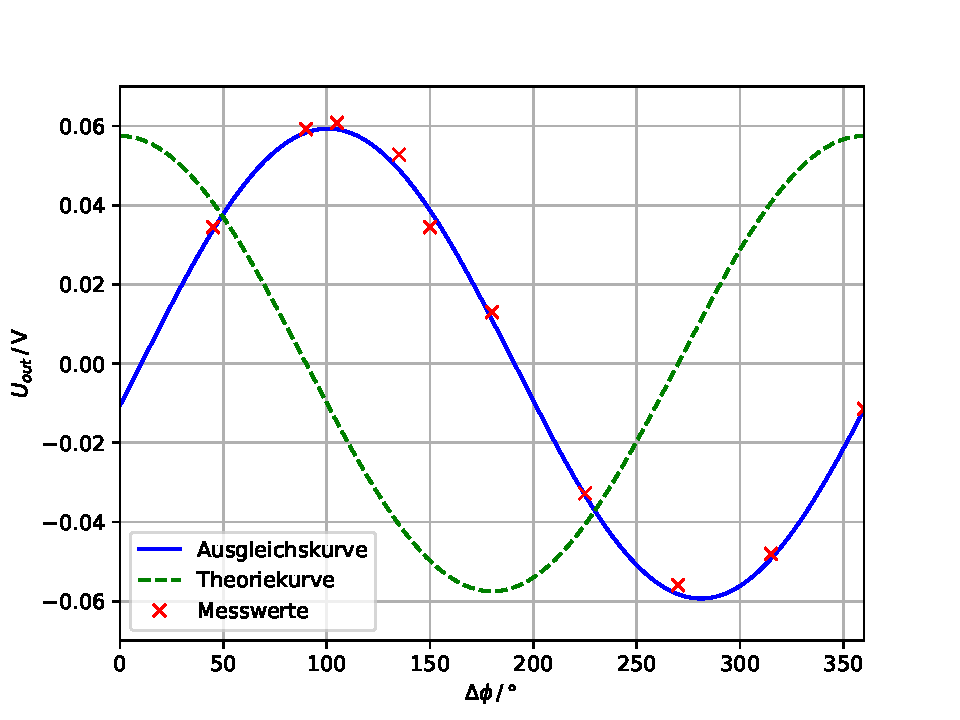
\includegraphics[width=\linewidth-75pt,height=\textheight-75pt,keepaspectratio]{content/images/plot2.pdf}
\caption{Graphen der Messwerte mit Tiefpassfilter mit Rauschen.}\label{fig:U4}
\end{figure}


\subsubsection{Leuchtdiode}
Die Pulsfrequenz der LED wurde auf $\SI{200}{\hertz}$ und die Verstärkung am Vorverstärker auf 50 eingestellt. Die gemessenen Werte der Spannung $U$ bei verschiedenen Abständen $r$ sind in Tabelle \ref{tab:tab3} zu sehen.
\begin{table}
	\centering
	\caption{Messwerte der Ausgangsspannung $U_.{out}$ nach dem Tiefpassfilter mit Rauschen.}
	\sisetup{table-format=1.2}
	\begin{tabular}{S[table-format=3.0] S[table-format=2.2]}
		\toprule
		{$r/10^2/\si[per-mode=reciprocal]{\metre}$}&{$U/\si[per-mode=reciprocal]{\volt}$} \\
		\midrule
		30 & 11,20 \\
		34 & 9,00 \\
		38 & 7,40 \\
		42 & 6,17 \\
		46 & 5,25 \\
		50 & 4,49 \\
		54 & 3,92 \\
		58 & 3,36 \\
		62 & 2,98 \\
		66 & 2,65 \\
		70 & 2,32 \\
		74 & 2,05 \\
		78 & 1,83 \\
		82 & 1,62 \\
		86 & 1,45 \\
		90 & 1,37 \\
		94 & 1,26 \\
		98 & 1,16 \\
		102 & 1,08 \\
		106 & 1,00 \\
		110 & 0,93 \\
		114 & 0,86 \\
		118 & 0,80 \\
		122 & 0,74 \\
		126 & 0,70 \\
		130 & 0,65 \\
		134 & 0,60 \\
		138 & 0,51 \\
		\bottomrule
	\end{tabular}
	\label{tab:tab3}
\end{table}

\noindent In Abbildung \ref{fig:U5} ist U gegen r aufgetragen.

\begin{figure}
\centering
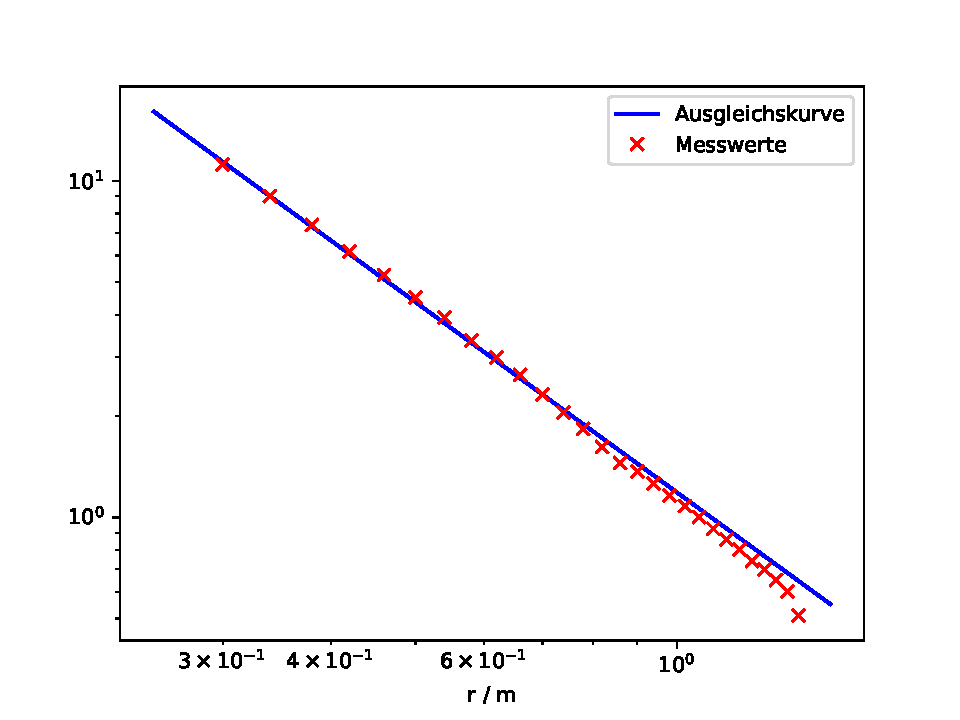
\includegraphics[width=\linewidth-75pt,height=\textheight-75pt,keepaspectratio]{content/images/plot3.pdf}
\caption{Logarithmische Darstellung des Verhaltens der Spannung bei zunehmendem Abstand der Leuchtdiode.}\label{fig:U5}
\end{figure}

\noindent Mittels der Regression $U(r)=a\cdot r^{-b}$ ergibt sich
\[
b_.{gemessen}=1,88\pm 0,02 \text{.}
\]
Der theoretische Wert für $b$ liegt bei 
\[
b_.{theo}=2 \text{.}
\]
Somit beträgt die Abweichung
\[
\Delta b = 5,95 \% \text{.}
\]